% \iffalse
\let\negmedspace\undefined
\let\negthickspace\undefined
\documentclass[beamer]{IEEEtran}
\usepackage{cite}
\usepackage{amsmath,amssymb,amsfonts,amsthm}
\usepackage{algorithmic}
\usepackage{graphicx}
\usepackage{textcomp}
\usepackage{xcolor}
\usepackage{txfonts}
\usepackage{listings}
\usepackage{enumitem}
\usepackage{mathtools}
\usepackage{gensymb}
\usepackage{comment}
\usepackage[breaklinks=true]{hyperref}
\usepackage{tkz-euclide} 
\usepackage{listings}
\usepackage{gvv}                                        
\def\inputGnumericTable{}                                 
\usepackage[latin1]{inputenc}                                
\usepackage{color}                                            
\usepackage{array}                                            
\usepackage{longtable}                                       
\usepackage{calc}                                             
\usepackage{multirow}                                         
\usepackage{hhline}                                           
\usepackage{ifthen}                                           
\usepackage{lscape}
\usepackage[export]{adjustbox}

\newtheorem{theorem}{Theorem}[section]
\newtheorem{problem}{Problem}
\newtheorem{proposition}{Proposition}[section]
\newtheorem{lemma}{Lemma}[section]
\newtheorem{corollary}[theorem]{Corollary}
\newtheorem{example}{Example}[section]
\newtheorem{definition}[problem]{Definition}
\newcommand{\BEQA}{\begin{eqnarray}}
\newcommand{\EEQA}{\end{eqnarray}}
\newcommand{\define}{\stackrel{\triangle}{=}}
\theoremstyle{remark}
\newtheorem{rem}{Remark}
\begin{document}
\parindent 0px
\bibliographystyle{IEEEtran}

\title{Assignment\\[1ex]10.5.4-2}
\author{ee23btech11215 - Penmetsa Srikar Varma$^{}$% <-this % stops a space
}
\maketitle
\newpage
\bigskip

\renewcommand{\thefigure}{\theenumi}
\renewcommand{\thetable}{\theenumi}
\section*{Question:}
Q2) The sum of the third and the seventh terms of AP is 6 and their product is 8. Find the sum of first sixteen terms of the AP\\
\section*{Solution:}
{
\centering
Table of Parameters\\
}
\begin{table}[h]
    \centering
    \begin{tabular}{|c|c|}
    \hline
     Input Variables & Input Condition \\
\hline
     x\brak{2}+x\brak{6}& 6 \\
\hline
     x\brak{2}.x\brak{6} & 8 \\
\hline
     $x_i$\brak{n} &  general term of $\text{i}^\text{th}$ AP sequence\\
\hline
     $y_i$\brak{n} &  sum of first n terms of $\text{i}^\text{th}$ AP sequence\\
\hline
     $x_i$\brak{0} & first term of $\text{i}^\text{th}$ AP sequence\\
\hline
     $d_i$ & common difference of $\text{i}^\text{th}$ AP sequence\\
\hline
    \end{tabular}
    \label{table of parameters}
\end{table}
Then from table of parameters,
\begin{align}
x_i^2\brak{6}-6\ x_i\brak{6}+8&=0
\end{align}
\begin{align}
x_i\brak{6}&=2\ or\ 4
\end{align}
\begin{enumerate}
 \item \begin{align}
    \brak{\ x_i\brak{2},x_i\brak{6}\ } &=
    \begin{cases}
        \brak{2,4} & \text{if } i = 1 \\
        \brak{4,2} & \text{if } i = 2 
    \end{cases}
\end{align}
\item \begin{align}
    \brak{\ x_i\brak{0},d_i\ }&=
    \begin{cases}
         \brak{1,\frac{1}{2}}& \text{if } i=1 \\
         \brak{5,-\frac{1}{2}} & \text{if } i=2
    \end{cases}
\end{align}
\item \begin{align}
    x_i\brak{n} &=
    \begin{cases}
        \brak{\frac{n+2}{2}}u\brak{n} & \text{if } i=1 \\
        \brak{\frac{10-n}{2}}u\brak{n} & \text{if } i=2 
    \end{cases}
\end{align}
\end{enumerate}
$z$-Transform of $x_1\brak{\text{n}}$ is given by:
\begin{align} X_1\brak{z}&=\frac{1-\frac{z^{-1}}{2}}{\brak{1-z^{-1}}^2},\quad |z^{-1}|<1
\end{align}
Similarly,
\begin{align}X_2\brak{z}&=\frac{5-\frac{11z^{-1}}{2}}{\brak{1-z^{-1}}^2},\quad |z^{-1}|<1 \end{align}
Similarly for sum of first n terms of AP,
\begin{align}
y_i\brak{n}&=x_1\brak{n}*u\brak{n}
\end{align}
\begin{align}
\label{w1}
Y_i\brak{z}&=\frac{X_i\brak{z}}{\brak{1-z^{-1}}}
\end{align}
\begin{align}
Y_1\brak{z}&=\frac{1-\frac{z^{-1}}{2}}{\brak{1-z^{-1}}^3},\quad |z|>1
\end{align}
\begin{align}Y_2\brak{z}&=\frac{5-\frac{11z^{-1}}{2}}{\brak{1-z^{-1}}^3},\quad |z|>1\end{align}
\begin{figure}[h]
    \centering
    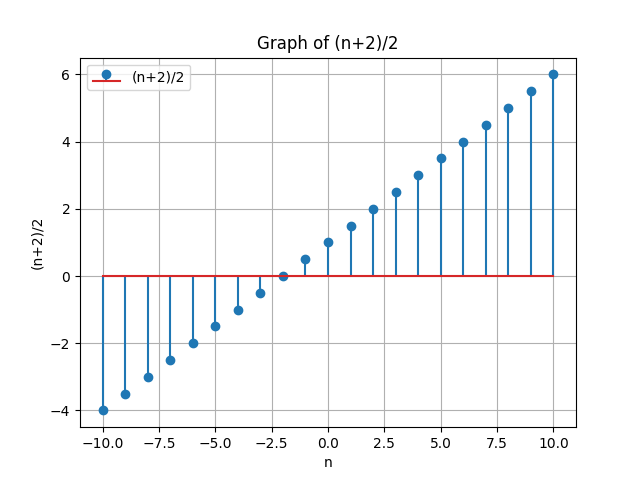
\includegraphics[scale=0.60]{py_3.png}
    \label{fig:x1n}
\end{figure}
\begin{center}
    Graph of $x_1\brak{n}$
\end{center}
\begin{figure}[h]
    \centering
    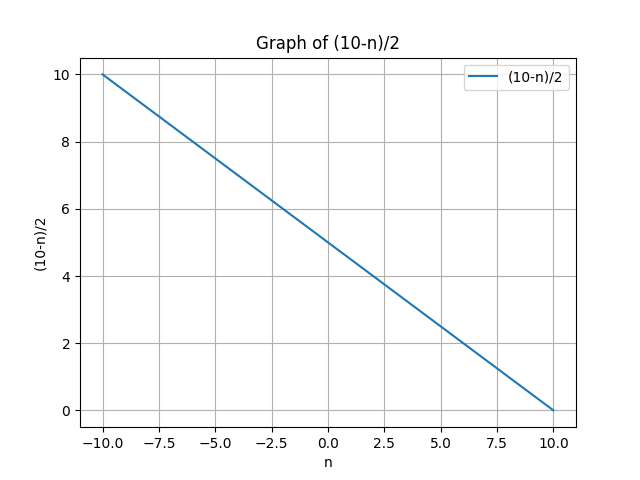
\includegraphics[scale=0.60]{py_5.png}
    \label{fig:x2n}
\end{figure}
\begin{center}
    Graph of $x_2\brak{n}$\\[20ex]
\end{center}
Inverse $z$-transform by counter integral method for  $y_1\brak{z}$,\\\\Since n starts from 0 to n-1 for $x_1\brak{n}$ so, n $\to$ n-1 so that $y_1\brak{n}$ starts from 1 to n for given n,\\
\begin{align}
y_1\brak{16}&=\oint_C \frac{z^3\brak{1-\frac{z^{-1}}{2}}}{\brak{z-1}^3}\ z^{14}\, dz
\end{align}
\begin{align}
y_1\brak{16}&=\frac{1}{2!}\brak{\frac{d^2}{dz^2}z^{17}-\frac{1}{2}\frac{d^2}{dz^2}z^{16}}_{z=1}  
\end{align}
\begin{align}
y_1\brak{16}&=76
\end{align}
Similarly for $y_2\brak{z}$,
\begin{align}
y_2\brak{16}&=\oint_C \frac{z^3\brak{5-\frac{11z^{-1}}{2}}}{\brak{z-1}^3}\ z^{14}\, dz
\end{align}
\begin{align}
y_2\brak{16}&=\frac{1}{2!}\brak{5\ \frac{d^2}{dz^2}z^{17}-\frac{11}{2}\frac{d^2}{dz^2}z^{16}}_{z=1}  
\end{align}
\begin{align}
y_2\brak{16}&=20
\end{align}
In fact,
\begin{align}
y_1\brak{n}&=\frac{n\brak{n+3}}{4}
\end{align}
\begin{align}
y_2\brak{n}&=\frac{n\brak{21-n}}{4}
\end{align}
\begin{figure}[h]
    \centering
    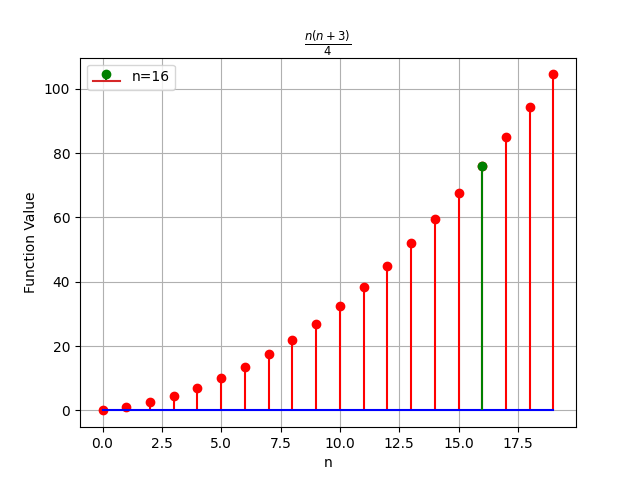
\includegraphics[scale=0.60]{py_4.png}
    \label{fig:s1n}
\end{figure}
\begin{center}
    Graph of $y_1\brak{n}$\\[30ex]
\end{center}
\begin{figure}[h]
    \centering
    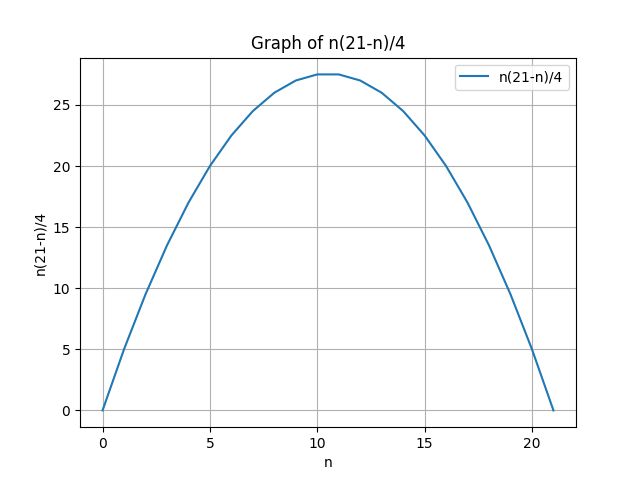
\includegraphics[scale=0.60]{py_6.png}
    \label{s2n}
\end{figure}
\begin{center}
Graph of $y_2\brak{n}$
\end{center}

\end{document}
